% !TEX program = xelatex
% 실험16 E — Gated Late Fusion 상세 흐름 (보고용, 한글).
%   ① 입력 모달리티 → 두 arm → 위험점수 표준화 → gate network → 가중합 → risk
%   ② gate network(b, c) 학습: inner CV 로 λ 선택 → 전체 학습 환자로 재학습 → 시험 환자 적용
%   ③ g = 2σ(c·z) 곡선: c = 0(게이트 꺼짐), 실제 학습된 최대 수준, 설명용 큰 c
% 수치 출처: experiments/실험16_GMU_nestedCV/nested_fusion/{model.py (GatedLateFusion), config.py},
%            outputs/gmu_nested/gated_nested/results.json (fold 별 λ, b, C).
\documentclass[tikz,border=8pt]{standalone}
\usepackage{fontspec}
\setmainfont{Noto Sans CJK KR}
\setsansfont{Noto Sans CJK KR}
\usepackage{amsmath,amssymb,graphicx}
\usetikzlibrary{positioning,arrows.meta,calc,fit,backgrounds}

% figstyle.tex 와 같은 팔레트 (폰트만 xelatex 용으로 바꿈)
\definecolor{navy}{HTML}{2F3B52}
\definecolor{ink}{HTML}{1A1A1A}
\definecolor{ink2}{HTML}{5A5E66}
\definecolor{boxblue}{HTML}{CFE0F7}
\definecolor{boxpink}{HTML}{F6CDD0}
\definecolor{boxpurple}{HTML}{DCD6F3}
\definecolor{boxyellow}{HTML}{FDEEB8}
\definecolor{boxgray}{HTML}{E9E9E9}
\definecolor{boxgreen}{HTML}{DCEFDC}
\definecolor{learn}{HTML}{D2691E}
\definecolor{stage}{HTML}{F5F6F8}

\tikzset{
  every node/.style={text=ink},
  blk/.style={draw=navy, line width=0.7pt, rounded corners=2.5pt, fill=#1,
              inner xsep=5pt, inner ysep=4pt, font=\small, align=center},
  blk/.default=boxgray,
  arr/.style={-{Latex[length=2.2mm,width=1.7mm]}, draw=navy, line width=0.8pt},
  lab/.style={font=\scriptsize, text=ink2, align=center, inner sep=1pt},
  op/.style={circle, draw=navy, line width=0.7pt, fill=white, inner sep=0pt,
             minimum size=5.5mm, font=\small},
  dot/.style={circle, fill=navy, inner sep=0pt, minimum size=1.6mm},
  flowstep/.style={blk=white, text width=3.25cm, minimum height=1.75cm, font=\footnotesize},
}
\newcommand{\lc}[1]{{\color{learn}#1}}   % 학습되는 값 표시

% 입력 아이콘 (figstyle.tex 와 같은 모양)
\newcommand{\iconimage}[2]{%
  \node[blk=boxblue, inner sep=1.1pt, minimum width=0pt, minimum height=0pt] (#1) at #2
       {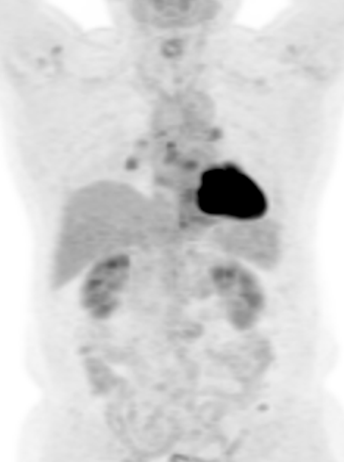
\includegraphics[height=11.8mm]{assets/pet_mip_icon.png}};%
}
\newcommand{\iconclinical}[2]{%
  \begin{scope}[shift={#2}]
    \begin{scope}
      \clip[rounded corners=2.5pt] (-5.25mm,-6mm) rectangle (5.25mm,6mm);
      \fill[boxpurple] (-5.25mm,-6mm) rectangle (5.25mm,6mm);
      \fill[navy!28]   (-5.25mm,3.3mm) rectangle (5.25mm,6mm);
      \draw[navy!45, line width=0.35pt]
        (-5.25mm,3.3mm) -- (5.25mm,3.3mm)  (-5.25mm,0.8mm) -- (5.25mm,0.8mm)
        (-5.25mm,-1.7mm) -- (5.25mm,-1.7mm) (-5.25mm,-4.2mm) -- (5.25mm,-4.2mm)
        (-1.75mm,-6mm) -- (-1.75mm,6mm)     (1.75mm,-6mm) -- (1.75mm,6mm);
    \end{scope}
    \draw[navy, line width=0.7pt, rounded corners=2.5pt] (-5.25mm,-6mm) rectangle (5.25mm,6mm);
    \node[minimum width=10.5mm, minimum height=12mm, inner sep=0pt] (#1) at (0,0) {};
  \end{scope}%
}
\newcommand{\iconreport}[2]{%
  \begin{scope}[shift={#2}]
    \fill[boxpink] (-4.6mm,-6mm) -- (-4.6mm,6mm) -- (1.7mm,6mm) -- (4.6mm,3.1mm) -- (4.6mm,-6mm) -- cycle;
    \draw[navy, line width=0.7pt, rounded corners=1pt]
      (-4.6mm,-6mm) -- (-4.6mm,6mm) -- (1.7mm,6mm) -- (4.6mm,3.1mm) -- (4.6mm,-6mm) -- cycle;
    \fill[navy!20] (1.7mm,6mm) -- (1.7mm,3.1mm) -- (4.6mm,3.1mm) -- cycle;
    \draw[navy, line width=0.55pt] (1.7mm,6mm) -- (1.7mm,3.1mm) -- (4.6mm,3.1mm);
    \draw[navy!55, line width=0.5pt]
      (-2.9mm,1.4mm) -- (2.9mm,1.4mm)  (-2.9mm,-0.4mm) -- (2.9mm,-0.4mm)
      (-2.9mm,-2.2mm) -- (2.9mm,-2.2mm) (-2.9mm,-4.0mm) -- (0.9mm,-4.0mm);
    \node[minimum width=9.2mm, minimum height=12mm, inner sep=0pt] (#1) at (0,0) {};
  \end{scope}%
}

\begin{document}
\begin{tikzpicture}[x=1cm,y=1cm]

% =====================================================================
% 제목
% =====================================================================
\node[anchor=west, font=\Large\bfseries] at (-2.3,6.3) {Gated Late Fusion: 입력에서 위험점수(risk)까지};
\node[anchor=west, font=\small, text=ink2] at (-2.3,5.7)
  {OS, PFS 각각 따로 학습. \lc{주황색} = gate network 단계에서 학습되는 값 ($b$ 2개 + $c$ 4개 = 6개)};

% ---------------- 단계 배경 ----------------
\begin{scope}[on background layer]
  \fill[stage, rounded corners=5pt] (-2.3,-1.75) rectangle (8.55,4.95);
  \fill[boxgreen!40, rounded corners=5pt] (8.75,-1.75) rectangle (22.3,4.95);
\end{scope}
\node[anchor=north west, font=\small\bfseries, text=ink2] at (-2.15,4.85) {Stage 1. 두 모델을 각자 따로 학습 (학습 후 고정)};
\node[anchor=north west, font=\small\bfseries, text=ink2] at (8.9,4.85)  {Stage 2. Gate network로 두 점수를 환자마다 다르게 섞기};

% =====================================================================
% ① 입력 → arm → 표준화
% =====================================================================
% 영상 줄 (y = 3.0)
\iconimage{im}{(0,3.4)}
\node[lab, anchor=east] at (-0.75,3.4) {PET-CT\\ MIP};
\node[blk, minimum width=30mm] (ia) at (3.3,3.4) {\textbf{Image arm}\\ {\scriptsize SimpleCNN $\to$ Cox head}};
\node[blk, minimum width=17mm, font=\footnotesize] (si) at (6.9,3.4) {표준화\\ {\scriptsize $(r-\mu)/\sigma$}};

% tabular 줄 (y = 0)
\iconclinical{cl}{(0,0.75)}
\iconreport{rp}{(0,-0.75)}
\node[lab, anchor=east] at (-0.7,0.75)  {임상\\ 19변수};
\node[lab, anchor=east] at (-0.7,-0.75) {판독지\\ 텍스트};
\node[blk, minimum width=30mm, minimum height=16mm] (ta) at (3.3,0) {\textbf{Tabular arm}\\ {\scriptsize 임상 MLP $\oplus$ RadBERT--MLP}\\ {\scriptsize $\to$ Cox head}};
\node[blk, minimum width=17mm, font=\footnotesize] (st) at (6.9,0) {표준화\\ {\scriptsize $(r-\mu)/\sigma$}};

\draw[arr] (im) -- (ia);
\draw[arr] (cl.east) -- (cl.east -| ta.west);
\draw[arr] (rp.east) -- (rp.east -| ta.west);
\draw[arr] (ia) -- node[above, font=\small] {$r_{\text{img}}$} (si);
\draw[arr] (ta) -- node[above, font=\small] {$r_{\text{tab}}$} (st);
\node[lab] at (6.9,1.7) {$\mu,\sigma$: 학습 환자에서만 계산};

% =====================================================================
% ② gate network → 곱하기 → 합 → risk
% =====================================================================
\node[font=\small] (zi) at (9.55,3.4) {$z_{\text{img}}$};
\node[font=\small] (zt) at (9.55,0)   {$z_{\text{tab}}$};
\draw[arr] (si) -- (zi);  \draw[arr] (st) -- (zt);

% gate network
\node[blk=white, draw=navy, line width=1pt, text width=4.9cm, minimum height=2.15cm, align=left] (gn) at (13.2,1.7)
  {\textbf{Gate network}\\[3pt]
   $g_{\text{img}} = 2\,\sigma(\lc{c_{21}}\,z_{\text{tab}} + \lc{c_{22}}\,z_{\text{img}})$\\[2pt]
   $g_{\text{tab}} = 2\,\sigma(\lc{c_{11}}\,z_{\text{tab}} + \lc{c_{12}}\,z_{\text{img}})$\\[3pt]
   {\scriptsize\color{ink2} $c$는 모든 환자 공통.}\\ {\scriptsize\color{ink2} 입력 $z$가 환자마다 달라서 $g$도 환자마다 다름}};

% z 줄과 gate 연결
\node[dot] (ti) at (10.4,3.4) {};
\node[dot] (tt) at (10.4,0)   {};
\draw[arr] (ti) -- (ti |- gn.north);
\draw[arr] (tt) -- (tt |- gn.south);

% λ: 학습할 때만 c 크기를 누르는 벌점 (예측 흐름에는 없음)
\node[blk=white, draw=learn, dashed, line width=0.8pt, font=\scriptsize, inner ysep=3pt] (lam) at (13.95,4.1)
  {\textbf{\color{learn}$\lambda$} {\color{learn}(학습할 때만)}: $c$가 커지지 않게 누르는 벌점 \;→\; $\lambda$가 크면 $c\approx0$, $g\approx1$};
\draw[-{Latex[length=2mm,width=1.6mm]}, draw=learn, dashed, line width=0.8pt] (lam.south) -- (lam.south |- gn.north);

% 곱하기 노드
\node[op] (mi) at (16.4,3.4) {$\times$};
\node[op] (mt) at (16.4,0)   {$\times$};
\draw[arr] (zi) -- (mi);
\draw[arr] (zt) -- (mt);
\draw[arr] ($(gn.east)+(0,0.55)$) -- (16.4,2.25) -- node[right, font=\small] {$g_{\text{img}}$} (mi.south);
\draw[arr] ($(gn.east)+(0,-0.55)$) -- (16.4,1.15) -- node[right, font=\small] {$g_{\text{tab}}$} (mt.north);

% b 곱하기
\node[blk=boxyellow, minimum width=12mm, font=\small] (bi) at (18.2,3.4) {$\times\,\lc{b_{\text{img}}}$};
\node[blk=boxyellow, minimum width=12mm, font=\small] (bt) at (18.2,0)   {$\times\,\lc{b_{\text{tab}}}$};
\draw[arr] (mi) -- (bi);  \draw[arr] (mt) -- (bt);

% 합 → risk
\node[op] (sm) at (19.8,1.7) {$+$};
\draw[arr] (bi.east) -| (sm.north);
\draw[arr] (bt.east) -| (sm.south);
\node[blk=boxyellow, font=\small\bfseries, minimum height=9mm] (rk) at (21.35,1.7) {risk};
\draw[arr] (sm) -- (rk);
\node[lab, anchor=north] at (19.35,-0.65)
  {$\text{risk} = \lc{b_{\text{tab}}}\,g_{\text{tab}}\,z_{\text{tab}} + \lc{b_{\text{img}}}\,g_{\text{img}}\,z_{\text{img}}$};
\node[lab, anchor=north] at (19.35,-1.1) {$c$가 모두 0이면 $g=1$ $\Rightarrow$ 기존 late fusion과 같은 식};

% =====================================================================
% ③ gate network 학습 과정 (outer fold 마다)
% =====================================================================
\node[anchor=west, font=\normalsize\bfseries] at (-2.3,-2.55)
  {Gate network ($b$, $c$) 학습 과정 — outer fold 5개마다 반복, 시험 환자는 쓰지 않음};

\node[flowstep] (s1) at (-0.55,-4.25)
  {\textbf{1. 입력 준비}\\ 학습 환자(약 190명)의\\ inner OOF 점수\\ $z_{\text{tab}}, z_{\text{img}}$};
\node[flowstep] (s2) at (3.35,-4.25)
  {\textbf{2. $\lambda$ 후보 비교}\\ $\lambda\in\{0.01, 0.1, 1, 10, 100\}$\\ 각각 inner 4-fold로\\ 학습 → 검증 C-index 평균};
\node[flowstep] (s3) at (7.25,-4.25)
  {\textbf{3. $\lambda$ 선택}\\ 평균 C-index가\\ 가장 높은 $\lambda$\\ (동점이면 큰 $\lambda$)};
\node[flowstep] (s4) at (11.15,-4.25)
  {\textbf{4. 최종 학습 → 평가}\\ 고른 $\lambda$로 학습 환자\\ 전체에서 \lc{$b$, $c$} 재학습\\ → 시험 환자(약 48명) 적용};
\draw[arr] (s1) -- (s2);  \draw[arr] (s2) -- (s3);  \draw[arr] (s3) -- (s4);

% 손실 함수
\node[blk=boxyellow!60, text width=14.65cm, align=center, font=\small] (loss) at (5.3,-6.05)
  {학습 손실 $=$ Cox 부분우도 손실 (Efron) $\;+\;\lambda\,(\lc{c_{11}}^2+\lc{c_{12}}^2+\lc{c_{21}}^2+\lc{c_{22}}^2)$\\[1pt]
   {\footnotesize\color{ink2}L-BFGS로 \lc{$b$}, \lc{$c$}를 함께 학습. $\lambda$는 학습할 때만 쓰이고 예측할 때는 쓰이지 않음}};
\draw[arr, dashed] (s2.south) -- (s2.south |- loss.north);
\draw[arr, dashed] (s4.south) -- (s4.south |- loss.north);

% λ 의 역할
\node[blk=white, text width=6.95cm, align=left, font=\footnotesize, anchor=north west] at (-2.3,-6.75)
  {\textbf{$\lambda$가 크면} (예: 100)\\ $c$를 키우면 벌점이 커짐 → $c\approx0$ → 모든 환자 $g\approx1$\\ → \textbf{게이트가 꺼지고 late fusion과 같아짐}};
\node[blk=white, text width=6.95cm, align=left, font=\footnotesize, anchor=north west] at (5.35,-6.75)
  {\textbf{$\lambda$가 작으면} (예: 0.1)\\ $c$가 0에서 멀어질 수 있음\\ → \textbf{환자마다 $g$가 달라짐} (환자별 게이팅)};

% 실험16 결과
\node[blk=boxgray, text width=14.65cm, align=left, font=\footnotesize, anchor=north west] at (-2.3,-8.35)
  {\textbf{실험16 결과}\quad 선택된 $\lambda$ — OS: 1, 100, 0.1, 1, 0.1 \;/\; PFS: 1, 100, 0.1, 100, 1 (fold 1--5)\\
   학습된 $c$는 모두 $|c|\le0.15$ → 게이트 값이 대부분 1 근처 (가장 크게 움직인 OS fold 3도 $g_{\text{img}}$ 0.77--1.15)};

% =====================================================================
% ④ g 곡선 예시
% =====================================================================
\begin{scope}[shift={(16.85,-6.9)}]
  \def\sx{0.72} \def\sy{1.45}
  \node[anchor=west, font=\small\bfseries] at (-1.0,4.25) {$c$ 크기에 따른 게이트 값 예시};
  \node[anchor=west, lab] at (-1.0,3.8) {$g_{\text{img}}=2\,\sigma(c\cdot z_{\text{img}})$, \;$z_{\text{tab}}=0$인 환자};
  % 축
  \draw[navy!30, line width=0.4pt] ({-3*\sx},{1*\sy}) -- ({3*\sx},{1*\sy});
  \draw[navy!30, line width=0.4pt] ({-3*\sx},{2*\sy}) -- ({3*\sx},{2*\sy});
  \draw[navy, line width=0.6pt] ({-3*\sx},0) -- ({3*\sx},0);
  \draw[navy, line width=0.6pt] ({-3*\sx},0) -- ({-3*\sx},{2.15*\sy});
  \foreach \v in {0,1,2} \node[anchor=east, font=\scriptsize, text=ink2] at ({-3*\sx-0.05},{\v*\sy}) {\v};
  \foreach \v in {-2,0,2} \node[anchor=north, font=\scriptsize, text=ink2] at ({\v*\sx},-0.05) {\v};
  \node[anchor=north, lab] at (0,-0.4) {환자의 $z_{\text{img}}$ (영상 위험점수, 표준화)};
  \node[lab, rotate=90, anchor=south] at ({-3*\sx-0.4},{1*\sy}) {$g_{\text{img}}$};
  % 곡선
  \draw[ink2, line width=1.6pt] ({-3*\sx},{1*\sy}) -- ({3*\sx},{1*\sy});
  \draw[learn, line width=1.4pt, domain=-3:3, samples=40, smooth]
       plot ({\x*\sx}, {\sy*2/(1+exp(0.15*\x))});
  \draw[navy!70, line width=1.2pt, dashed, domain=-3:3, samples=60, smooth]
       plot ({\x*\sx}, {\sy*2/(1+exp(-1.0*\x))});
  % 범례
  \draw[ink2, line width=1.6pt] (-1.0,-1.05) -- +(0.45,0); \node[anchor=west, font=\scriptsize] at (-0.5,-1.05) {$c=0$: 모든 환자 $g=1$ (게이트 꺼짐)};
  \draw[learn, line width=1.4pt] (-1.0,-1.45) -- +(0.45,0); \node[anchor=west, font=\scriptsize] at (-0.5,-1.45) {$c=-0.15$: 실험16에서 학습된 최대 수준};
  \draw[navy!70, line width=1.2pt, dashed] (-1.0,-1.85) -- +(0.45,0); \node[anchor=west, font=\scriptsize] at (-0.5,-1.85) {$c=1$: $c$가 컸다면 (설명용 가정)};
\end{scope}

\end{tikzpicture}
\end{document}
